\documentclass[a4paper, 13pt]{extarticle}
\usepackage{graphicx}
\usepackage[margin=2.5cm]{geometry}
\graphicspath{{images/}}
\usepackage{amsmath}
\usepackage{titlesec}
\titlelabel{\thetitle.\quad}
\usepackage{color}
\usepackage{caption}
\usepackage{subcaption}
\usepackage{parskip}
\usepackage{helvet}
\usepackage{hyperref}
\usepackage[T1]{fontenc}
\usepackage{mathptmx}
\usepackage{setspace}
\usepackage{lipsum}
\usepackage{listings}
\usepackage{pgf,tikz,pgfplots}
\usepackage{mathrsfs}
\usepackage{xfrac}
\usetikzlibrary{arrows}



\renewcommand{\baselinestretch}{1.5} 
\begin{document}



\begin{titlepage}

  \newcommand{\HRule}{\rule{\linewidth}{0.5mm}} % Defines a new command for the horizontal lines, change thickness here

  \center % Center everything on the page

%	HEADING SECTION

  %\textsc{\LARGE University Name}\\[1.5cm] % Name of your university/college
  \text{\Large UNIVERSITY OF SCIENCE AND TECHNOLOGY OF HANOI}\\[0.3cm] % Major heading such as course name
  \textsc{\bfseries UNDERGRADUATE SCHOOL}\\[1.2cm] % Minor heading such as course title
  
\includegraphics[scale = 0.1]{usth.png}\\[1cm]
  \text{ \large Research and Development}\\[0.5cm]
    {\LARGE \bfseries BACHELOR THESIS}  \\ [1cm]
    \text{\large By}\\[0.3cm]
  \text{ \large Bui Vu Huy}\\[0.3cm]
  \text{ \large USTHBI7-082}\\[0.3cm]
  \text{\large Information and Communication Technology }\\[0.5cm]
  
  %	TITLE SECTION
  
  \vspace{1 cm}
  \HRule\\[0.5cm]

  \textbf{\fontsize{18}{20} \bfseries Virtual World Development using Unity Engine}\\[0.3cm] % Title of your document
    \HRule\\[0.5cm]

  
  %	AUTHOR SECTION
  
  \text{\large Supervisor:    Dr. Nguyen Hoang Ha}\\
  
  %	DATE SECTION
  
  \vspace{2.5 cm}
  \textbf{\large Hanoi, \today}\\[3cm] % Date, change the \today to a set date if you want to be precise
  
  
  \vfill % Fill the rest of the page with whitespace
  
\end{titlepage}
\newpage
\part*{\Large Table of Contents}

\newpage

\newpage
\section*{\color{cyan}\Large Acknowledgements}

First of all, i would like to thanks Dr.Nguyen Hoang Ha for giving me 3 months for using the Unity Engine to develop the Virtual World. Also, thank you for supporting me during this internship. 

I also thanks for the USTH ICT Lab for giving me a opportunities to work in a places like in a professional company. 

Finally, I'd like to give special thanks to the guys, girls who made free 3d models, characters in the Unity assets store, so that i can download, use them for my project.
\newpage
 
 \newpage
 \appendix
  \renewcommand{\thesubsection}{\Alph{section}}
 \renewcommand{\thesubsection}{\arabic{subsection}}
\section{\Large Introduction} 
Nowsadays, the technology is getting better and better, so the human life are becoming more and more convenient. With that, people's entertainment needs are also increasing. However, to satisfy people's needs, also to keep up with this rapid development of technology, a virtual world is also a type of entertainment that can satisfy people's need. \\[0.35cm]  A virtual world is a computer-base environment that the user can interact with each other in the world. In general, the virtual world usually using 3-dimensional graphic, with 3D models, which can make people feel like they're in the real world. Virtual worlds allow for multi user to communicate, and a 3D video single player game like Elder Scroll: Blade and Skyrim can still be consider as the virtual world. \\[0.35cm] In general term, there's still no generally accepted definition for virtual world, it supports varying degrees of play and gaming. These are some uses of term: MMOGs game: large number of players within a game, and RPG game, etc... \\[0.35cm] To create a virtual world, there're some types of engine that allow you to make like Unity, Unreal Engine, blender, etc... \\[0.35cm] From one of those engines, Unity is the most popular choice for many people, from beginner to expert. \\[0.35cm] Unity is a cross-platform game engine developed by Unity Technologies, first announced and released in June 2005 at Apple Inc.'s Worldwide Developers Conference as a Mac OS X-exclusive game engine. As of 2018, the engine had been extended to support more than 25 platforms. The engine can be used to create three-dimensional, two-dimensional, virtual reality, and augmented reality games, as well as simulations and other experiences. \\[0.35cm]
 In my opinion, first of all, it has tons of online tutorials to be found, the document with clean format, so a good step for beginners. With it's very intuitive design, C\# language make it easier to use or learn, like you can call other script within a script. Also, with great community, when you have a problem, they'll have you everywhere and every time. Unity has clean API, which is easy to use, understand, implement in C\# code, the application works very well on windows, Linux, android or iOS. Lastly, unlike other engines, the unity has asset store with lots of free assets for everyone to use, while the other ones only have few free assets. \\[0.35cm]In this work, i'll focus on creating the virtual world using unity engine, in particular, it's an RPG game, where you as a player can walk around, interact with other NPC model in the world, or attack some enemy that get in your way. 
  

 To create the virtual world with Unity, first, we'll need to create the terrain by the tools Unity provides for us. After that, we can create my own model and then just simply drag and drop the model into the scene, if not, there're several websites i can get free 3d model from like turbosquid or free3d. For the Lighting and the shadow, Unity also has build-in tool just like other engines, which can help me create the light and shadow easily, adjust it as i want. Furthermore, to make things look good, we can apply some textures to all the objects, prefabs. We can find the texture on google, choose the suitable one for a specific object, and then just simply drag and drop them on that object, or making our own texture. Finally, in order to move around or interact with the object, a camera and player controller should be added into the scene, however, Unity already has the FPScontroller prefab which can be found in the standard assets, we can use it directly without doing anything, but it's still possible to create the character controller from scratch with C\# code.
 \section{\Large Objective} 
 	In this project, since it's about building an RPG game, which is also a type of virtual world, I'll only focus on how to make the player move around the world, is able to interact with other objects around him. In this game, there may be some enemies that get in the way, the player should eliminate them which hurt the player. 
 \section{\Large Aim} 
 	The aim is not necessarily on destroying the enemies, but focus on completing 
 	the quest that villagers in the village gave the player. When finishing a quest, the player should return back to the village, talk to the villagers that you're finished. Beside that, the game should also have an online chat tab , which you can chat with other players who are connecting to the same network while playing game, they may help you finishing the quest faster. 

 
 
 \setcounter{secnumdepth}{4}
 \titleformat{\paragraph}
 {\normalfont\normalsize\bfseries}{\theparagraph}{1em}{}
 \titlespacing*{\paragraph}
 {0pt}{1.25ex plus 1ex minus .2ex}{1.5ex plus .2ex}
 
 \vspace{0.35 cm}
  \section{\Large Programs, Materials and Methods}
  	\subsection{External programs used}
  		\subsubsection{3DS Max}
 		 3DS Max, a program developed by Autodesk, previously called 3D Studio Max, is a 3D computer graphics program for making 3D animations, models , images...
 		 This program was used in this project in order to edit UV mapping of some models, correct the position of the texture. 
 		 \subsubsection{Photoshop}
 		 Photoshop is a photo editing and graphic design software. It is developed by Adobe Systems for MacOS and Windows. It's not like other graphic design or photo editing softwares, it can create normal map, height map, occulusion map from a single texture. With this, this software will help me with the technique bump mapping, so the game's texture will look more realistic. 
 		 \subsubsection{Visual Studio}
 		 Visual studio is an IDE (integrated development environment ) from Microsoft. It's used to develop computer programs, as well as websites, supports many programming languages such as : C++, C\#, JavaScript, etc... 
 		 This is the main software of this project, because i'm using this one to write scripts in order to make the game works.
 		 When installing unity 5, normally it's shipped with visual studio community which is free for everyone. Previously, it's shipped with the monodevelop, but now the monodevelop is discontinued, no longer support unity, replaced with visual studio community as it's more powerful than monodevelop, it support MacOS and windows, gives you a cloud storage for saving like one drive(when you project goes wrong), which monodevelop doesn't have.  
 		
 		 
 		 
 		 \subsection{Materials}
 		 \subsubsection{DirectX}
 		 DirectX is the collection of API (or  application programming interfaces), also made by Microsoft, for handling task related to multimedia. It contains these APIs such as Direct3D, DirectDraw, DirectMusic, DirectSound .... , especially for game programming. \\[0.15cm] The DirectX version use in this project here is Direct X11 because from unity 4.x or higher, the engine tend to use more cpu cores, and with Direct3D 11, it has improved multi-threading support so it can utilize multi-core better. Without Direct X, the engine cannot simulate the light in the game or even run. 
 		 \subsubsection{A dedicated graphic card}
 		 A graphic card with direct x11 compatible is compulsory for Unity. Because unity comes with MSAA support, to improve image, textures quality, which direct x10 or lower doesn't support. Integrated GPU is fine also as long as it's powerful enough to run unity programs, games and have direct x11 compatible. 
 		 
 		 \subsection{Method}  
 		 \subsubsection{Overview Diagram}
 		 - In this section, i'd like to introduce my overview diagram about the concept of creating a virtual world: \par
 		 
 		 	\begin{figure}[h]
 		 		\centering
 		 		\includegraphics[width=0.59\columnwidth]{Overview_diagram.png}
 		 		\captionof{figure}{Overview Diagram}
 		 		\label{fig:Overview1}
 		 	\end{figure}
 		 
 		 
 		 \newpage
 		  \subsubsection{Details}
 		  \paragraph{Preparation}
 		  Unity can be download from the \href{https://store.unity.com/}{offical website}. I prefer Unity personal version because it's free, for everyone. As i mentioned before, to be able to run Unity, and create a new project, you'll need at least direct x11 for simulate lighting, shadows on the scene. To create a terrain, which is the base of the virtual world, all i have to do is go to game object -> 3D Object -> Terrain. The terrain width and length is only set to 500x500, which i think is big enough for this project.  \begin{figure}[h]
 		  	\centering
 		  	\begin{minipage}{.4\textwidth}
 		  		\centering
 		  		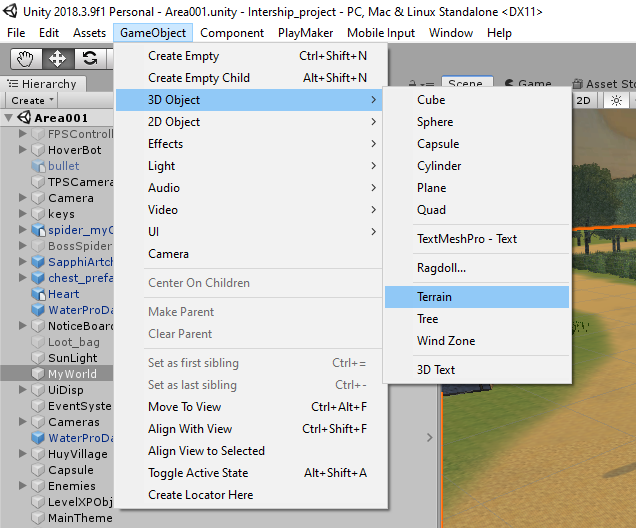
\includegraphics[width=1\linewidth]{intructions/1.png}
 		  		\captionof{figure}{Create terrain}
 		  		\label{fig:test2}
 		  	\end{minipage}
 		  	\begin{minipage}{.4\textwidth}
 		  		\centering
 		  		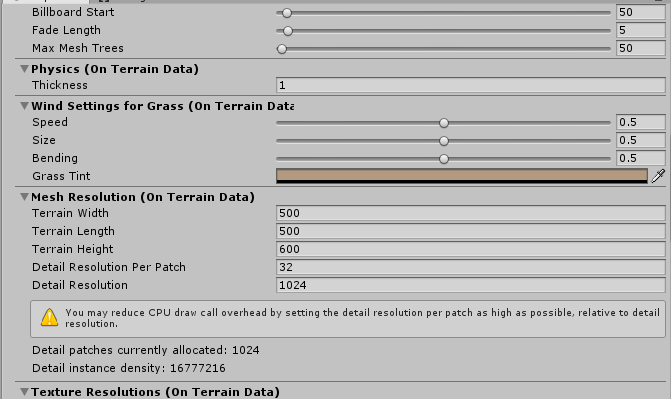
\includegraphics[width=1.4\linewidth]{intructions/2.png}
 		  		\captionof{figure}{Properties}
 		  		\label{fig:test3}
 		  	\end{minipage}
 		  \end{figure}
 	  \\[0.15cm]
 	  From the Inspector section, there're 4 sections: Paint texture, paint trees, paint details. Each of these sections has painting tool with 20 brush presets, resizable brush size, opacity. For the textures, you can use any texture you want for the terrain, for example i use this texture from this website: \href{https://www.textures.com/download/grass0153/48704}{https://www.textures.com/download/grass0153/48704}. The same applied for painting details, but for painting trees, the material for this one is 3D model, however it can be found in the Standard Assets which comes with Unity when installed. 
 	   \begin{figure}[h]
 	   	 \centering
 	   	 \begin{minipage}{1\textwidth}
 	   	 	\centering
 	   	 	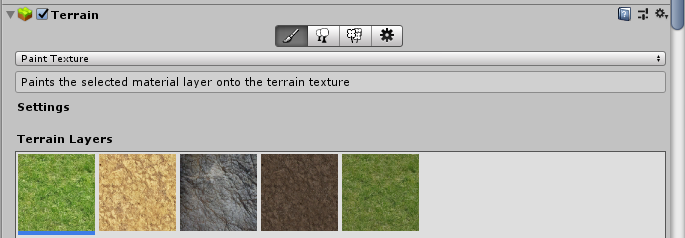
\includegraphics[width=0.75\linewidth]{intructions/3.png}
 	   	 	\captionof{figure}{Sections}
 	   	 	\label{fig:test4}
 	   	 \end{minipage}
 		 \end{figure}  
 		 
 	Besides, in order to make the terrain looks better, the user can also raise or lower the terrain to create mountains, river. After i finish creating the terrain, all i have to do is drag and drop other objects/prefabs into the scene, put the textures corresponding to each object, while these prefabs/objects can be found on unity assets store or from free3d website as i mentioned from the introduction. 
 	 \paragraph{Player}
 	 To be able to interact with the objects, NPCs, a player should be added into the scene. For example, i use this little robot for my player, this model is free to download, use: \href{https://free3d.com/3d-model/bb8-35865.html}{https://free3d.com/3d-model/bb8-35865.html}.
 	 
 	 \begin{figure}[h]
 	 	\centering
 	 	\begin{minipage}{1\textwidth}
 	 		\centering
 	 		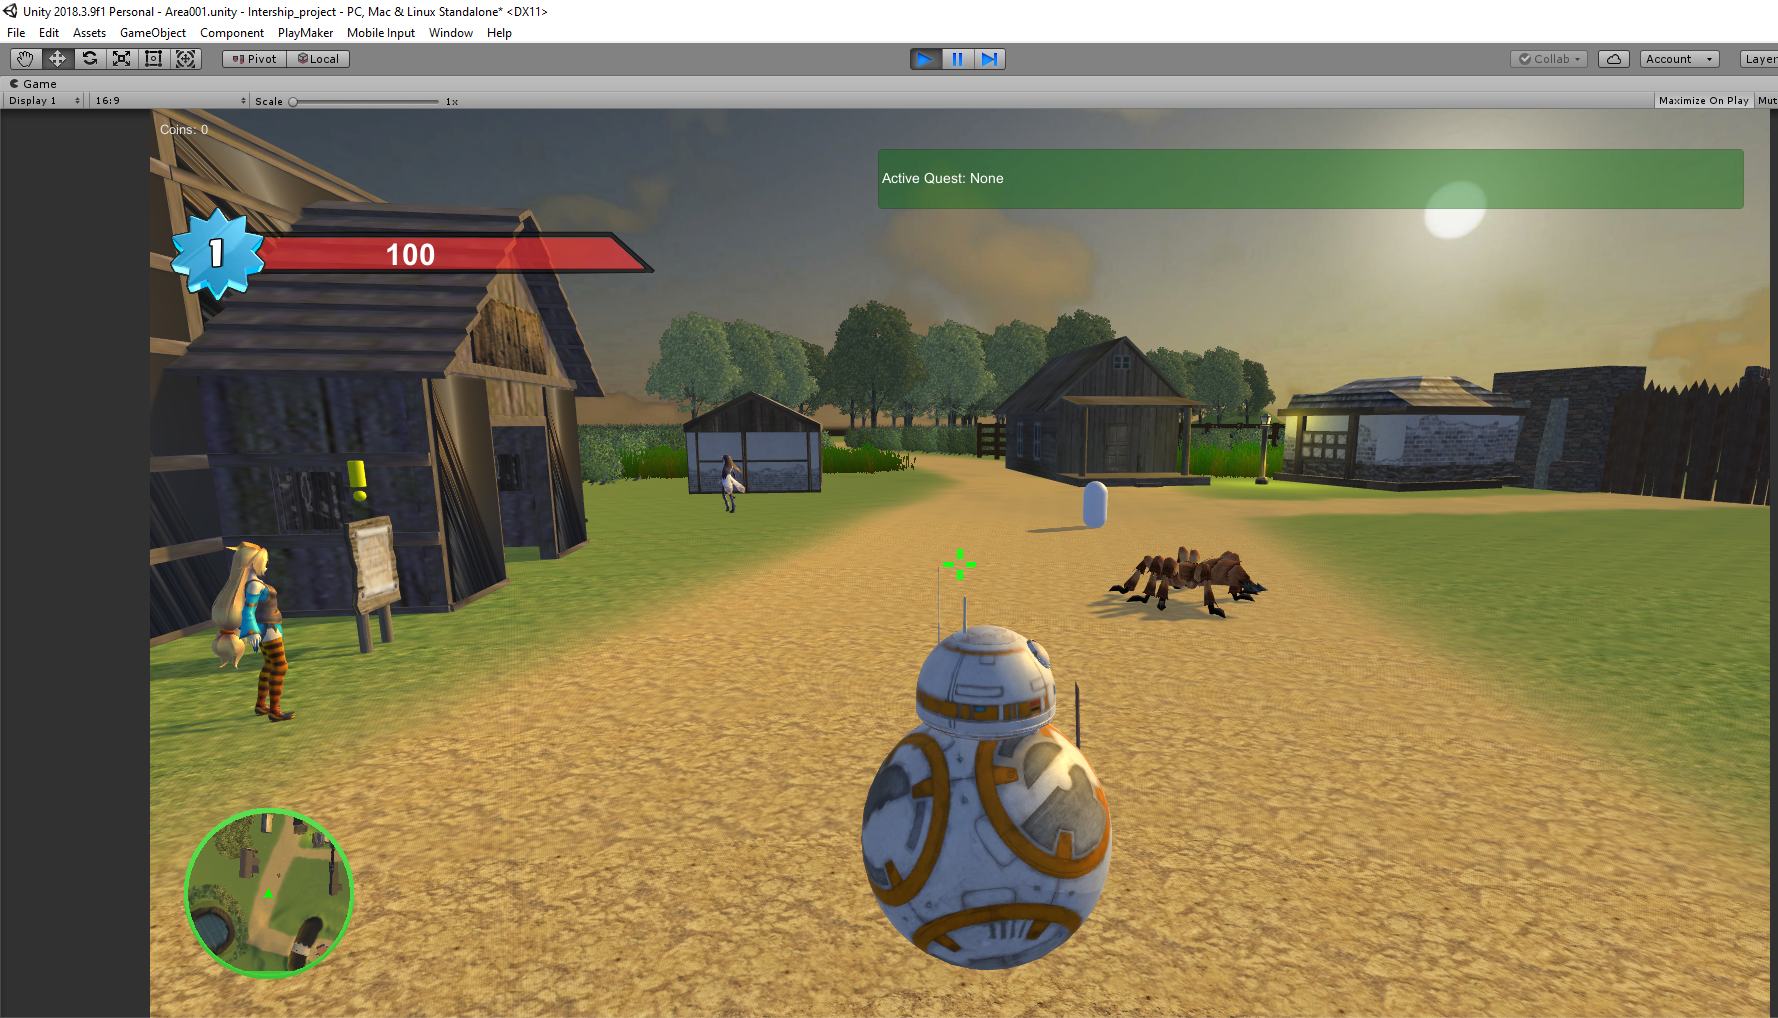
\includegraphics[width=0.75\linewidth]{intructions/4.png}
 	 		\captionof{figure}{Character example}
 	 		\label{fig:test5}
 	 	\end{minipage}
 	 \end{figure}
 	  
 	 Initially, the player will not move without any scripts attached to it, so i write a simple C\# script to control the player using visual studio and then attach the script to the player. Although there's a character controller prefab in the Unity's standard asset, which can be used, controlled instantly without doing anything. In this project, i'll not use character controller prefab, so that i can easily customize my character controller script later. \\[0.25cm] By default, when initializing a unity project, there's already a camera called "Main camera", which is what the user can see from the game view in the hierarchy. This camera will not follow my character as i move, but i'll explain how to make the camera follow my character later.  
 	 \\[0.25cm] From now, i'm going to explain how can i implement character controller to move my character. Firstly, i have to find the input by go to Edit -> Project Settings -> Input. In the input section, as you can see, the Unity already implement 2 inputs named : "Horizontal" , "Vertical", along with Negative Button and Positive Button, and i can also add my own custom input in project setting. This is where i can move my character left and right, forward and backward. After finding the input, i can get the input by using: 
 	 \lstdefinestyle{customc}{
 	 	belowcaptionskip=1\baselineskip,
 	 	breaklines=true,
 	 	frame=L,
 	 	xleftmargin=\parindent,
 	 	language=C,
 	 	showstringspaces=false,
 	 	basicstyle=\footnotesize\ttfamily,
 	 	keywordstyle=\bfseries\color{green!40!black},
 	 	commentstyle=\itshape\color{purple!40!black},
 	 	identifierstyle=\color{blue},
 	 	stringstyle=\color{orange},
 	 }
  
  \lstset{style=customc}
 	 \begin{lstlisting}
 	  Vector2 input = new Vector2(Input.GetAxis("Horizontal"), 
 	  Input.GetAxis("Vertical"));
 	 \end{lstlisting}
 	 Next, i have to normalize the input vector to see which direction the player have to move , face correctly. To be more specify, let's consider two trigonometry below:
 	
 	 		\definecolor{qqwuqq}{rgb}{0.,0.39215686274509803,0.}
 	 		\definecolor{ffqqqq}{rgb}{1.,0.,0.}
 	 		\definecolor{uuuuuu}{rgb}{0.26666666666666666,0.26666666666666666,0.26666666666666666}
 	 		\begin{tikzpicture}[line cap=round,line join=round,>=triangle 45,x=0.5cm,y=0.5cm]
 	 		\clip(-17.62,-11.46) rectangle (13.08,6.28);
 	 		\draw [shift={(-10.3,-3.27)},line width=0.5pt,color=qqwuqq,fill=qqwuqq,fill opacity=0.10000000149011612] (0,0) -- (0.4233601239113539:0.6) arc (0.4233601239113539:49.49045192111633:0.6) -- cycle;
 	 		\draw [line width=0.5pt] (-14.36,-3.3)-- (-6.24,-3.24);
 	 		\draw [line width=0.5pt] (-10.3,-3.27) circle (2.030055417962771cm);
 	 		\draw [line width=0.5pt] (-10.3,-3.27)-- (-6.24,-3.24);
 	 		\draw [line width=0.5pt] (-10.33,0.79)-- (-10.27,-7.33);
 	 		\draw [line width=2.8pt,color=ffqqqq] (-10.3,-3.27)-- (-7.662654488417639,-0.1831069580342808);
 	 		\draw [line width=0.5pt] (-7.662654488417639,-0.1831069580342808)-- (-7.639990169721227,-3.2503447549486797);
 	 		\draw (-10.74,1.68) node[anchor=north west] {90};
 	 		\draw [line width=0.5pt] (1.77,-3.3) circle (2.030055417962771cm);
 	 		\draw [line width=0.5pt] (-2.25,-3.31)-- (5.87,-3.25);
 	 		\draw (-5.82,-2.98) node[anchor=north west] {0};
 	 		\draw (-15.86,-3.14) node[anchor=north west] {180};
 	 		\draw (-10.94,-7.76) node[anchor=north west] {270};
 	 		\draw (1.46,1.66) node[anchor=north west] {0};
 	 		\draw (6.42,-2.92) node[anchor=north west] {90};
 	 		\draw (1.28,-7.96) node[anchor=north west] {180};
 	 		\draw (-3.74,-3.02) node[anchor=north west] {270};
 	 		\draw [line width=2.8pt,color=ffqqqq] (1.77,-3.3)-- (1.7404368698694395,0.7600032045968739);
 	 		\draw [line width=0.5pt] (1.77,-3.3)-- (1.7995631301305606,-7.3600032045968735);
 	 		\begin{scriptsize}
 	 		\draw [fill=uuuuuu] (-10.3,-3.27) circle (2.0pt);
 	 		\draw[color=black] (-8.94,-3.55) node {$X$};
 	 		\draw[color=black] (-7.32,-1.87) node {$Y$};
 	 		\draw[color=qqwuqq] (-9.22,-2.87) node {$\alpha$};
 	 		\draw [fill=uuuuuu] (1.77,-3.3) circle (2.0pt);
 	 		\end{scriptsize}
 	 		\end{tikzpicture}
 	 	\\[0.02cm]
 	 	From the left one above, suppose that the red line is the input direction, X and Y are vertical and horizontal component. Now, i have to find the angle {$\alpha$} which is the direction the character will rotate, calculated as: 
 	 	\\[-0.5cm]
 	 	\[\alpha = arctan(\frac{Y}{X})\]
 	 	In Unity, however, if my character is facing forward, then it has the rotation of 0 (as seen from the right one), when facing right it has the rotation of 90 degree and so on. Let's call the rotation of character in unity is r, when looking at the two circle, it's clearly that r is calculated as: \\[-0.5cm]
 	 	 \[r = 90 - \alpha; \hspace{0.8cm} or \hspace{1.0cm} r = arctan(\frac{X}{Y})\] 
 	 	By C\# code:
 	 	\begin{lstlisting}
 	 	float targetRotation = Mathf.Atan2(inputDir.x, inputDir.y) * Mathf.Rad2Deg;
 	 	transform.eulerAngles = Vector3.up * Mathf.SmoothDampAngle(transform.eulerAngles.y, targetRotation, ref turnSmoothVelocity, turnSmoothTime);
 	 	\end{lstlisting}
 	 	
 	 	Where Mathf.SmoothDampAngle is the function that can gradually change an angle given in degrees towards a desired angle by turnSmoothTime (in second). The reason i use Vector3.up is because the character won't rotate up or fly straight to the sky.  \\[0.15cm] After that, to be able to move, transform.forward and Controller.Move is used here to move the character by a certain amount in the world space everytime when i press a button. \\[0.15cm] Finally, to finish setting up my character controller script, i have also added gravity, ability to jump for my character. From 10th grade, the equation to calculate the falling speed is defined as: 
 	 	\\[-0.5cm]
 	 	 \[v = \sqrt{2gh}\]
 	 	 where g is the gravity and h is the height the character begin to fall. As there's no air resistance in the game, this equation can be applied directly to the character through the script. For the ability to jump:
 	 	 \begin{lstlisting}
 	 	 if (controller.isGrounded)
 	 	 {
 	 	 float jumpVelocity = Mathf.Sqrt(-2 * gravity * jumping);
 	 	 VelocityY = jumpVelocity;
 	 	 }
 	 	 Vector3 velocity = transform.forward * currentSpeed + Vector3.up * VelocityY;
 	 	 controller.Move(velocity * Time.deltaTime);
 	 	 
 	 	 if (controller.isGrounded)
 	 	 {
 	 	 VelocityY = 0;  
 	 	 }
 	 	 \end{lstlisting}
 	 	 Where VelocityY is defined as the falling speed equation above. As soon the character hit the ground, the character won't be able to fall anymore, so i have to assign VelocityY = 0 when controller.isGrounded. 
 	 \paragraph{Cameras}
 	 \begin{itemize}
 	 	\item \bfseries TPSCamera (Third Person Camera) 
 	 \end{itemize}
 	 
 	 Without the camera following the character, i cannot see what happened to him when he move outside the camera view, so in this section, i'll make a script to force the camera follow the character. To do that, let's implement transform.position = Target.position - transform.forward * distFromTarget , where the Target variable is the character object. The reason why i minus with transform.forward * distFromTarget is because to make sure that the camera always behind the character, not in front of him. 
 	 \begin{figure}[h]
 	 	\centering
 	 	\begin{minipage}{.4\textwidth}
 	 		\centering
 	 		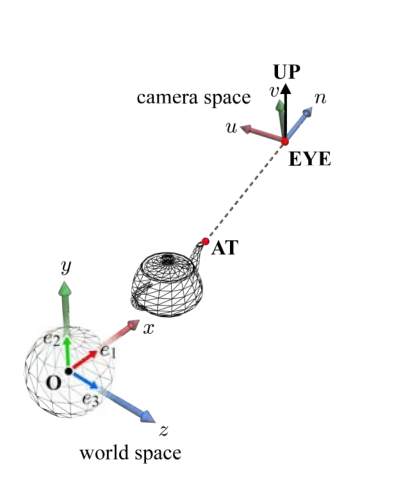
\includegraphics[width=0.7\linewidth]{intructions/camera_space.png}
 	 			\centering
 	 		\captionof{figure}{Camera world space}
 	 		\label{fig:test6}
 	 	\end{minipage}
  		\begin{minipage}{.4\textwidth}
  			\centering
  			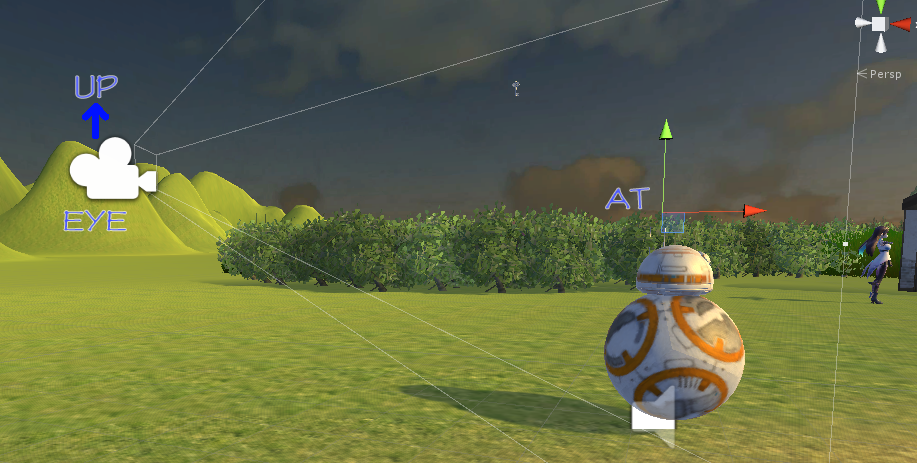
\includegraphics[width=1.2\linewidth]{intructions/my_camera_space.png}
  			\label{fig:test7}
  		\end{minipage}
 	 \end{figure}  
  	\\[0.05cm]
 	 The camera is specified in term of three parameters: {\bfseries EYE, AT}, and {\bfseries UP}, as show in the left one. EYE is the camera position , AT is the reference point the camera is pointing at, and UP usually is set to the y-axis of the world space. For example, in the right one, AT is set at the position a little bit above the character for not covering the crosshair at the middle of the screen.
 	 After that, the camera needed to be rotated around with a mouse because i'd like to see what is happening around the character. And the same applied to the character controller script, but this time, i use Input.GetAxisRaw function instead of GetAxis is because i don't want the rotating to be smooth immiately as it can cause a short delay as GetAxisRaw will only return 0,-1 or 1 while GetAxis change gradually from 0 to 1 or 0 to -1.  
 	 Moreover, the function Lerp is used here instead of SmoothDamp due to the fact that the smoothdamp function adds the curve which can cause delay, for example, when i stop moving my mouse, the camera still moving, while Lerp only behaves linear. As now, there's still one more problem, on the mouseY rotation, the camera can be rotated 360 degree which is not i wanted, so i used the function Mathf.Clamp to limit the rotation of the mouseY axis, the minimum, maximum here is -40, 85 degree for the third person camera controller. In the end, to finish my TPS camera controller, i've modified the charactercontroller script a bit by adding cameraT.eulerAngles.y in the targetRotation where cameraT is the MainCamera(the TPS camera), to make sure that the camera will following the player correctly.
 	 
 	  \begin{itemize}
 	 	\item \bfseries Camera Collision Detection 
 	 \end{itemize}
 	 
 	 	
 	 	
 	 	
  	\end{document}
	
 	 
 	 	
 	 
 	 
 	 